\documentclass[9pt]{beamer}
\usetheme{TUDOplain}
% workaround: provide commands not defiend by all bibtex styles
\providecommand{\btxandlong}{und}
\providecommand{\newblock}{}

\usepackage[english]{babel}
\usepackage[style=authortitle]{biblatex}
\addbibresource{../bibliography.bib}

% reformat footnotes very plain
\makeatletter
\renewcommand\@makefnmark{%
[\@thefnmark]}
\renewcommand\@makefntext[1]{%
  \noindent\tiny [\@thefnmark] #1}
\makeatother
% command for citing
\providecommand{\fcite}[1]{\footcite{#1}}
%

% basic utils
\usepackage[utf8]{inputenc}
\usepackage{enumerate}
\usepackage{graphicx}
\graphicspath{{../images/}}

\usepackage{ifthen}
\usepackage{calc}
\usepackage{amsmath,amsfonts,amssymb}
\setbeamertemplate{navigation symbols}{}
%\setbeamertemplate{footline}{}
%\setbeamertemplate{footline}[frame number]{}
\setbeamertemplate{footline}{\small \vspace{-1ex} \vbox{ \insertframenumber /\inserttotalframenumber}}
%\setbeamertemplate{footline}{\fontsize{7pt}{7pt}\selectfont \vspace{-1ex} \vbox{ \insertframenumber /\inserttotalframenumber}}

\author{Matthias Jakobs}
\title{End-to-end Human Activity Recognition framework on Complex Video Datasets}
\date{\today}
\institute[TU Dortmund]{Pattern Recognition In Embedded Systems,\\ Department of Computer Science \\ LS XII, Technische Universität Dortmund}
%
% frame command
\newenvironment{myframe}[1][]{%
\begin{frame}%
\frametitle{#1}
% start footnote numbers with 1
\setcounter{footnote}{0}


}{%
\end{frame}%
}

\begin{document}
\begin{frame}

\titlepage

% bst modified by A.Plinge to have consistent given family name order
% feel free to use others if required
%\bibliographystyle{gerabbrv3}
%  put all .bib files here
%\nobibliography{../bibliography}

\end{frame}

\section{Motivation}
\begin{myframe}[Motivation]
  \begin{figure}
    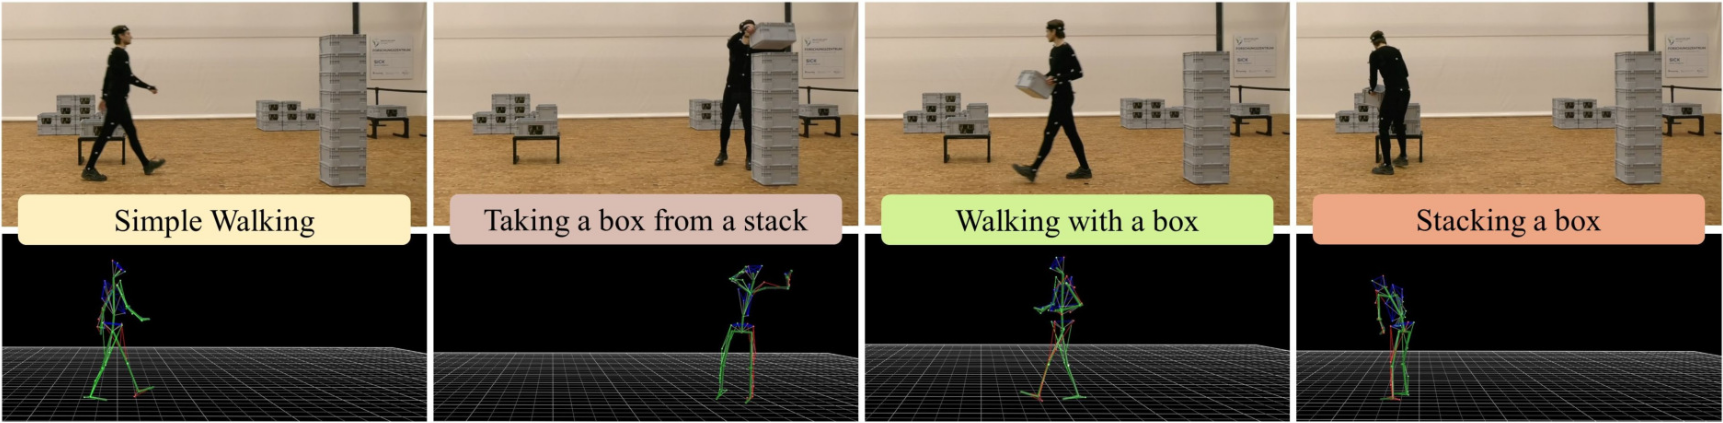
\includegraphics[width=\textwidth]{har-image-skeleton.png}
    \caption{Example of human activities in a warehouse context. Taken from \fcite{reining_towards_2018}}
  \end{figure}
  \begin{itemize}
      \item Motion capturing costly
      \item Pose estimators become better rapidly
      \item End-to-end training recently proposed
  \end{itemize}
\end{myframe}

\tableofcontents

\section{Fundamentals}
\subsection{Human Activity Recognition}

\begin{myframe}[Fundamentals - HAR]
    \begin{itemize}
        \item Identify action performed by human
        \item Multiple sources for detection
        \begin{itemize}
            \item Inertial Measurement Units (IMUs)
            \item Images (or video)
        \end{itemize}
    \end{itemize}
\end{myframe}

\begin{myframe}[Fundamentals - HAR]
    \begin{itemize}
        \item How fine-grained?
        \begin{itemize}
            \item \textit{Raising left arm} or
            \item \textit{Waving}
        \end{itemize}
    \end{itemize}
    $\Rightarrow$ \textit{attributes} vs. \textit{actions} \fcite{reining_towards_2018}
\end{myframe}

\subsection{Pose estimation}

\begin{myframe}[Fundamentals - Pose estimation]
    \begin{columns}[T]
        \begin{column}{0.45\textwidth}
            \vspace{30px}
            \begin{itemize}
                \item Detect joint locations
                \item Different definitions
                \item Single vs. multi person
                \item 2D and 3D methods
            \end{itemize}
        \end{column}
        \begin{column}{0.55\textwidth}
            \begin{figure}
                \includegraphics[width=.99\textwidth]{pe-singlehumna.png}
            \end{figure}
        \end{column}
    \end{columns}
    \begin{figure}
        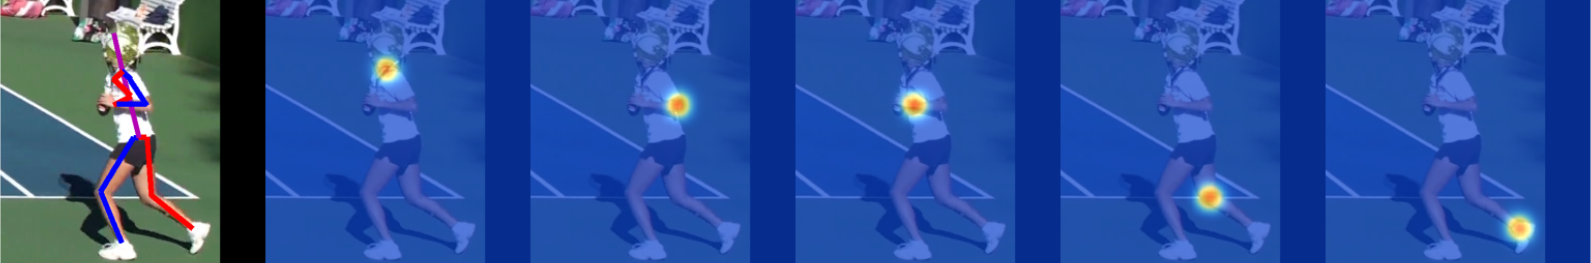
\includegraphics[height=50px]{2dheatmaps.png}
    \end{figure}
\end{myframe}

\begin{myframe}[Fundamentals - Pose estimation]
    \begin{figure}
        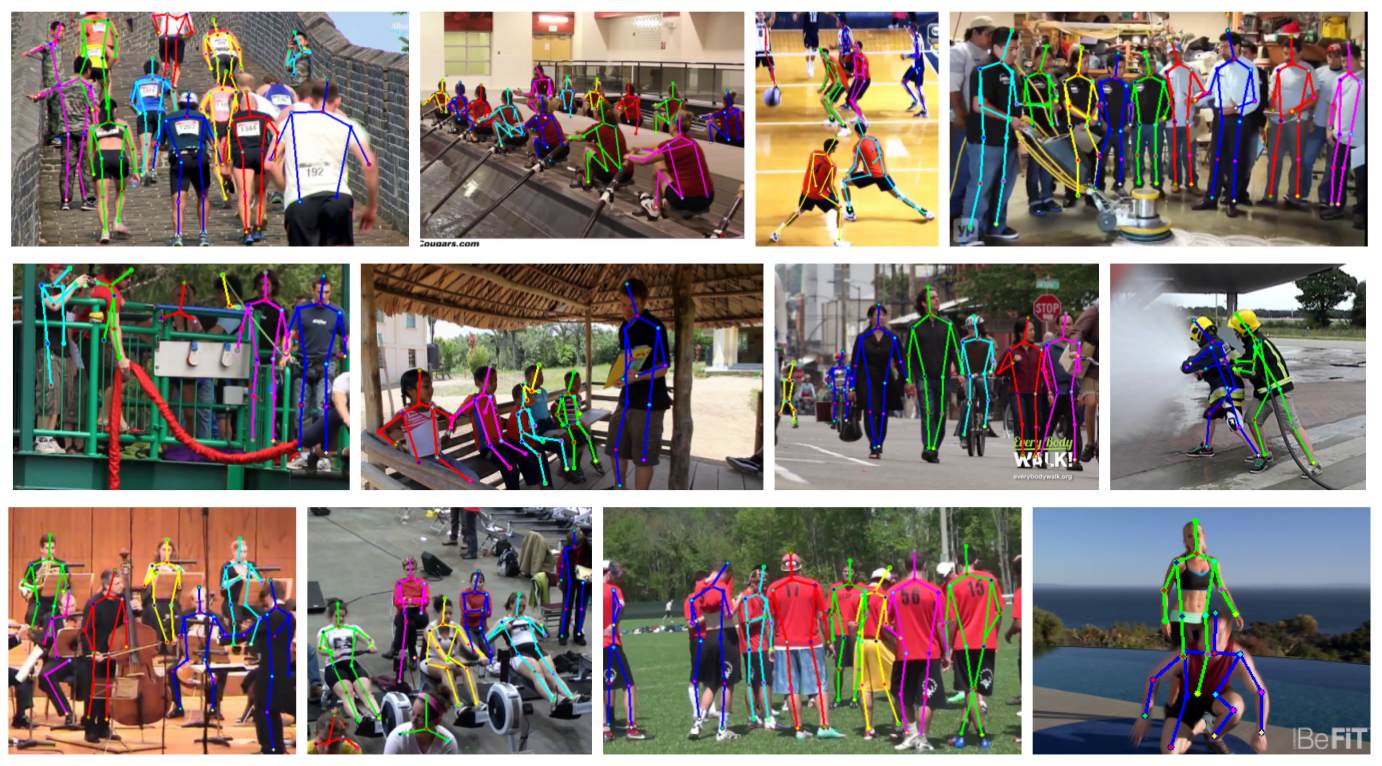
\includegraphics[width=.99\textwidth]{pe-multihuman.png}
    \end{figure}
\end{myframe}

\section{Related Work}
\subsection{2D / 3D pose estimation}

% \begin{myframe}[2D pose estimation]
%   \begin{itemize}
%     \item \textbf{shallow methods}
%     \begin{itemize}
%       \item Pictorial structure framework
%     \end{itemize}
%     \item \textbf{deep methods}
%     \begin{itemize}
%       \item Stacked hourglass \fcite{newell_stacked_2016}
%       \item Convolutional pose machine \fcite{wei_convolutional_2016}
%     \end{itemize}
%   \end{itemize}
% \end{myframe}
%
\begin{myframe}[Shallow methods]
    \begin{columns}[T]
        \begin{column}{.48\textwidth}
            \begin{itemize}
                \item \textbf{Pictorial structure framework \footnotemark\footnotemark\footnotemark}
              \begin{itemize}
                  \item Model human pose as tree of parts
                  \begin{itemize}
                      \item coordinates, size, orientation and type
                  \end{itemize}
                  \item Choose configuration with max score
                  \begin{itemize}
                      \item Learned from training data
                  \end{itemize}
              \end{itemize}
            \end{itemize}
        \end{column}
        \footnotetext[1]{\cite{fischler_representation_1973}}
        \footnotetext[2]{\cite{felzenszwalb_pictorial_2005}}
        \footnotetext[3]{\cite{yang_articulated_2011}}
        \begin{column}{.48\textwidth}
            \begin{figure}
                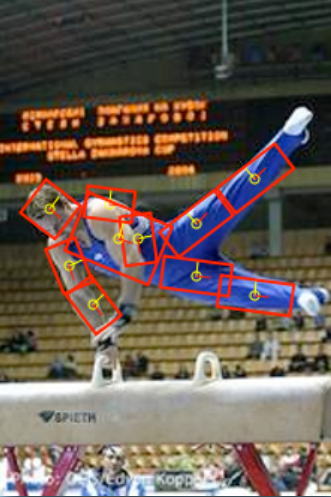
\includegraphics[height=150px]{pictoralexample.png}
            \end{figure}
        \end{column}
    \end{columns}
\end{myframe}

\begin{myframe}[2D pose estimation]
    \begin{columns}[T]
        \begin{column}{.48\textwidth}
            \begin{itemize}
                \vspace{25px}
                \item \textbf{Stacked hourglass network \footnotemark}
                  \begin{itemize}
                    \item Pooling, upsampling, skip-connections
                    \item Residual modules~\footnotemark
                    \item Refine result each block
                    \item Most SOTA methods build on top
                  \end{itemize}
            \end{itemize}
        \end{column}
        \footnotetext[1]{\cite{newell_stacked_2016}}
        \footnotetext[2]{\cite{he_deep_2016}}
        \begin{column}{.48\textwidth}
            \begin{figure}
                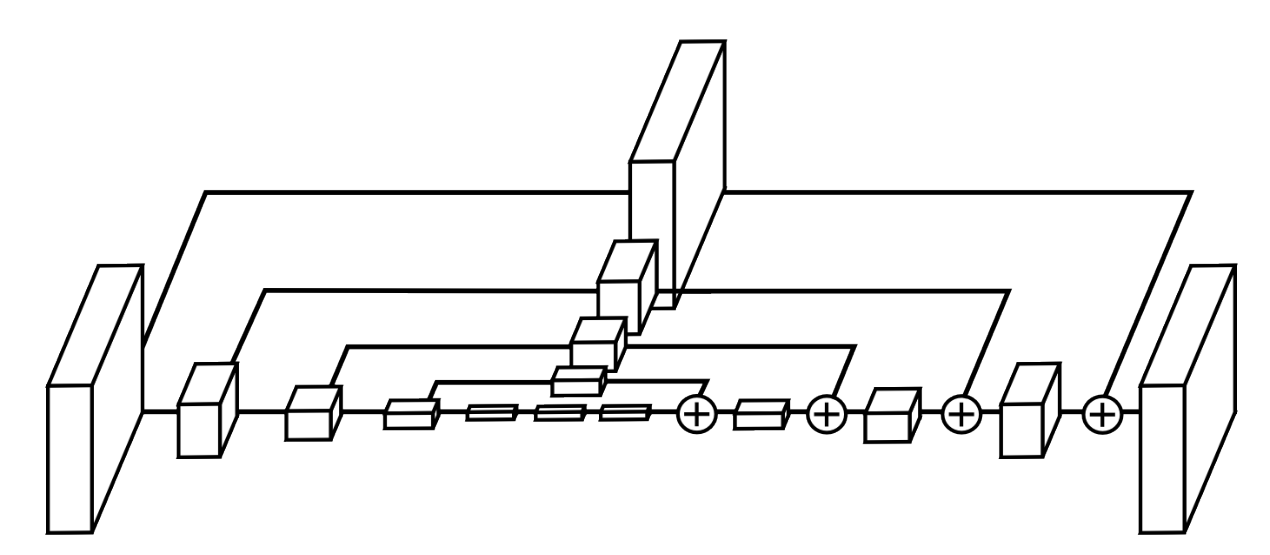
\includegraphics[width=.75\textwidth]{single-hourglass.png}
                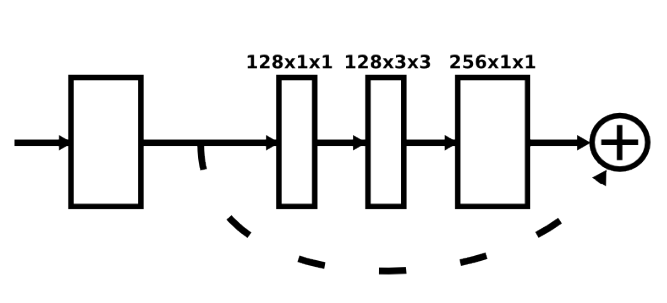
\includegraphics[width=.75\textwidth]{residualmodule.png}
            \end{figure}
        \end{column}
    \end{columns}
    \begin{figure}
        \includegraphics[width=.99\textwidth]{stackedhourglass.png}
    \end{figure}
\end{myframe}

\begin{myframe}[3D pose estimation]
    \begin{itemize}
        \item \textbf{Lifting}
        \begin{itemize}
            \item \textit{Convert} 2D coordinates into 3D
			\item Better results than end-to-end
			\begin{itemize}
				\item Predominant approach
			\end{itemize}
			\item Even simple approaches gain state-of-the-art \fcite{martinez_simple_2017}
        \end{itemize}
    \end{itemize}
\end{myframe}

% \subsection{Video-based HAR}
% \begin{myframe}[Video-based HAR]
%   \begin{itemize}
%     \item \textbf{shallow methods}
%     \begin{itemize}
%         \item Learning Realistic Human Actions from Movies \fcite{laptev_learning_2008}
%     \end{itemize}
%     \item \textbf{deep methods}
%     \begin{itemize}
%         \item Mixed Convolutional Tube \fcite{zhou_mict:_2018}
%     \end{itemize}
%     \item \textbf{joint, end-to-end methods}
%     \begin{itemize}
%         \item Multitask Deep Learning Framework \fcite{luvizon_2d/3d_2018}
%     \end{itemize}
%   \end{itemize}
% \end{myframe}

\begin{myframe}[Video-based HAR]
	\begin{itemize}
		\item \textbf{Learning Realistic Human Actions from Movies \fcite{laptev_learning_2008}}
		\begin{itemize}
			\item Spatio-temporal extension of Harris corner detection
			\item Volume around interest points
			\begin{itemize}
				\item \textit{HoG}
				\item \textit{HoF}
				\item concatenation and normalization
			\end{itemize}
			\item Clustering into BoF
		\end{itemize}
	\end{itemize}
	\begin{figure}
		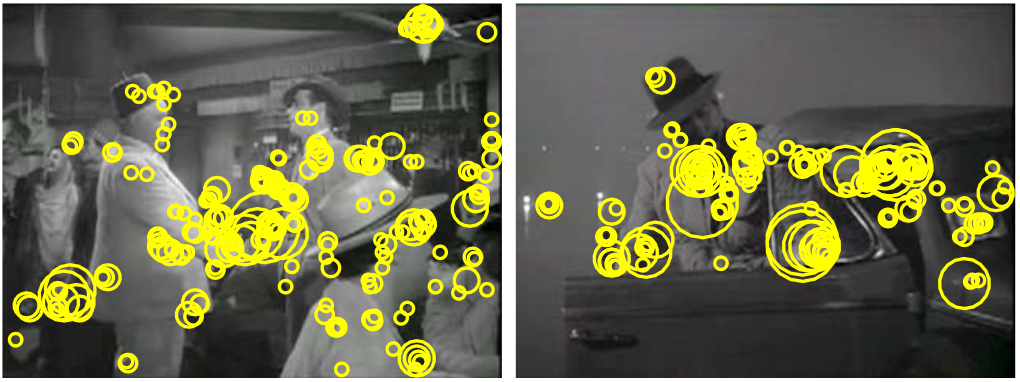
\includegraphics[width=.7\textwidth]{spacetimeinterestpoints.png}
		\caption{Left: Shaking hand, right: getting out of car.}
	\end{figure}
\end{myframe}

\begin{myframe}[Video-based HAR]
	\begin{itemize}
		\item \textbf{MiCT: Mixed Convolutional Tube \fcite{zhou_mict:_2018}}
		\begin{itemize}
			\item Third dimension $\Rightarrow$ temporal dimension
			\item Combining 2D and 3D convolutions more accurate than just 3D
			\item 4 MiCT blocks, followed by FC
			\item State-of-the-art on HMDB51 for RGB-only methods
		\end{itemize}
	\end{itemize}
	\begin{figure}
		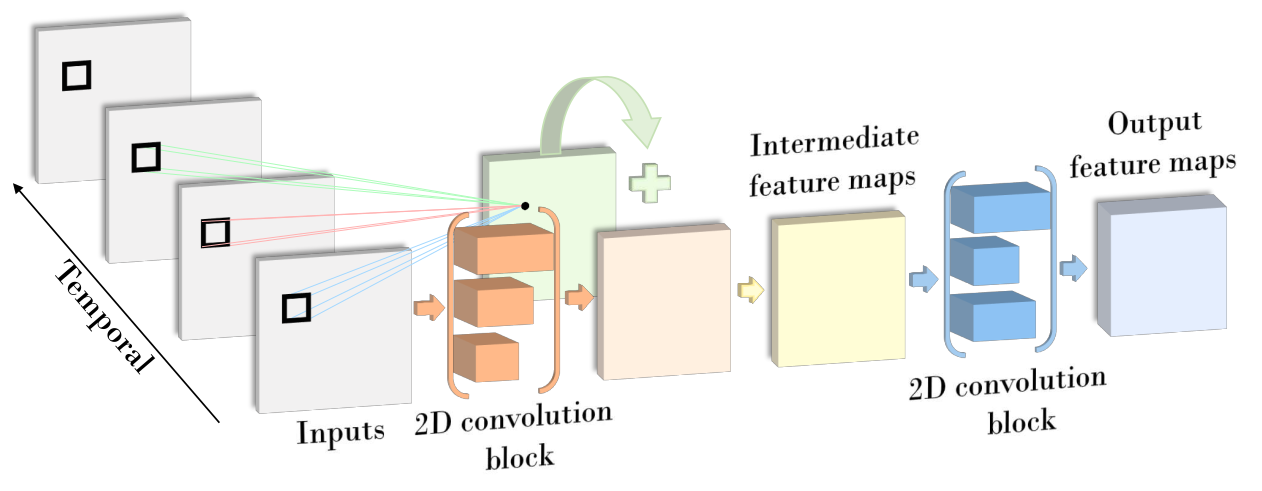
\includegraphics[width=.7\textwidth]{mict-block.png}
		\caption{Combining simple 2D convolutions with 3D convolutions}
	\end{figure}
\end{myframe}

\begin{myframe}[MiCT-Net]
	\begin{figure}
		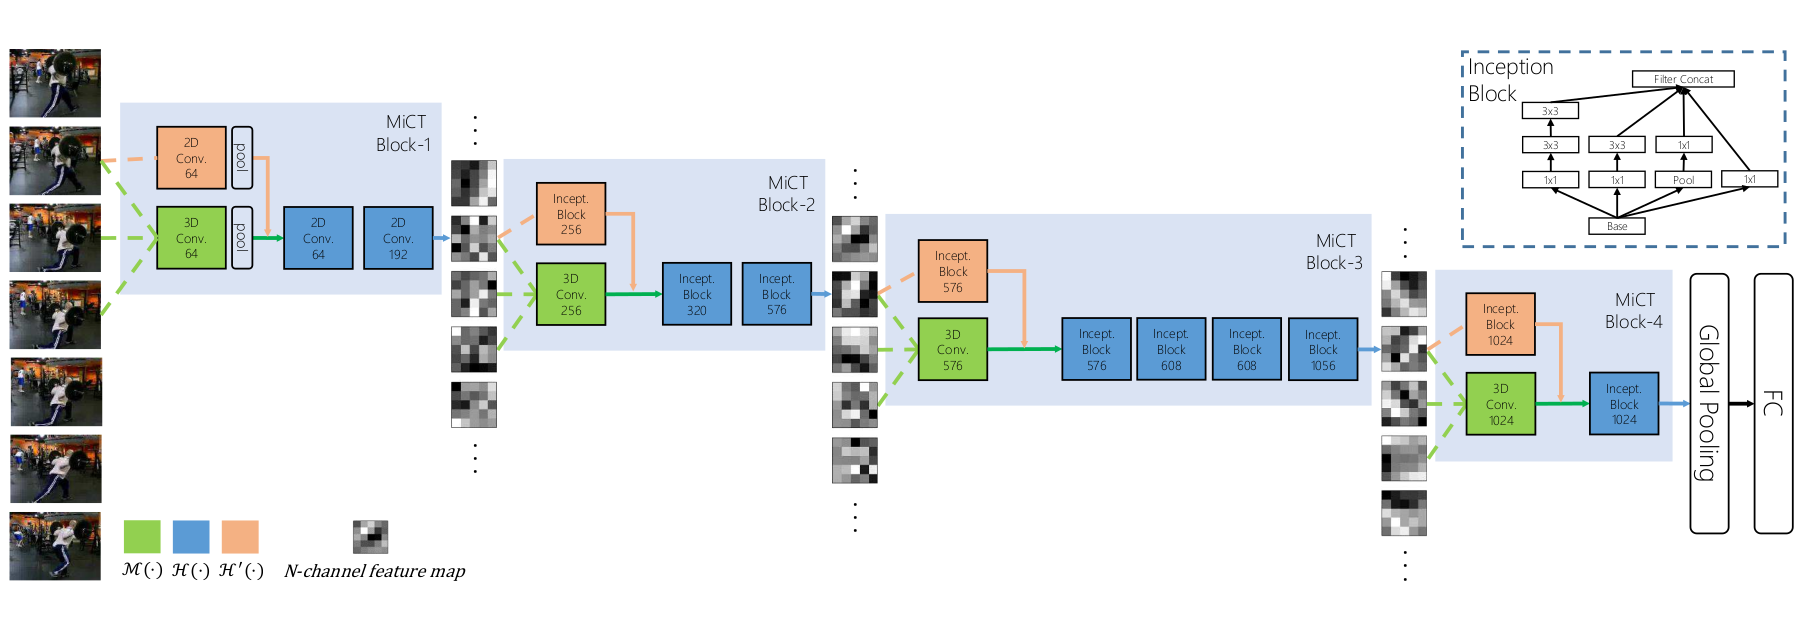
\includegraphics[width=.99\textwidth]{mict-full.png}
		\caption{Full architecture of MiCT-Net.}
	\end{figure}
\end{myframe}

\begin{myframe}[End-to-end pose and HAR frameworks]
	\begin{columns}[T]
	\begin{column}{.45\textwidth}
		\begin{itemize}
			\item \textbf{Multitask Deep Learning}\footnotemark
			\begin{itemize}
				\item \textit{Soft-argmax}\footnotemark~makes end-to-end learning possible
			\end{itemize}
		\end{itemize}
        \begin{figure}
            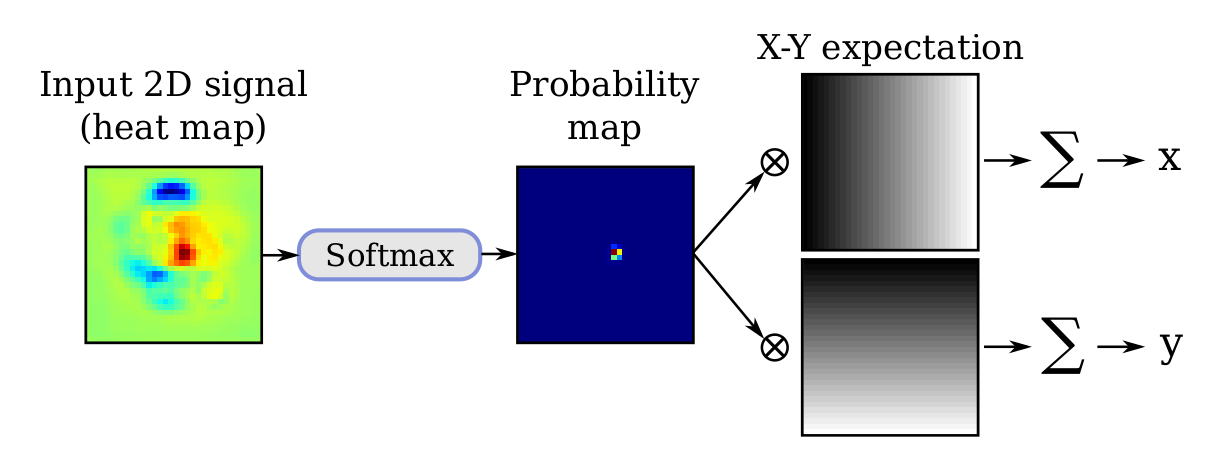
\includegraphics[width=0.99\textwidth]{softargmax.png}
            %\caption{Soft-argmax, graphical representation}
        \end{figure}
		\begin{figure}
            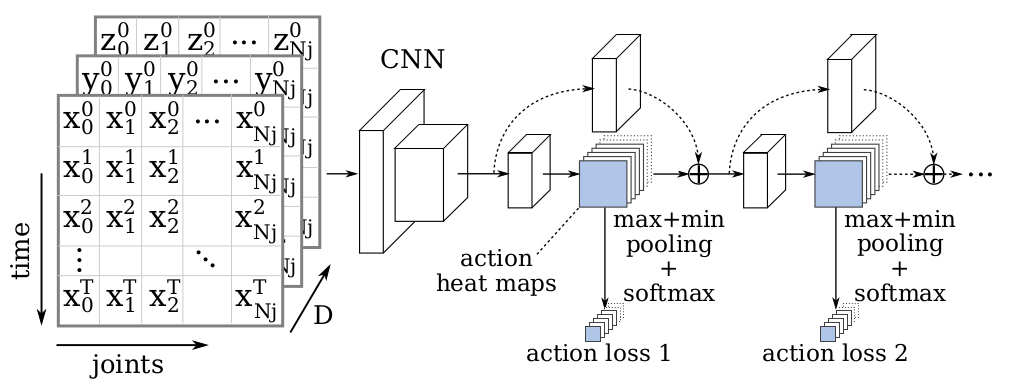
\includegraphics[width=.99\textwidth]{jointsovertime.png}
		\end{figure}
	\end{column}
    \footnotetext[1]{\cite{luvizon_2d/3d_2018}}
    \footnotetext[2]{\cite{luvizon_human_2017}}
	\begin{column}{.45\textwidth}
		\begin{figure}
			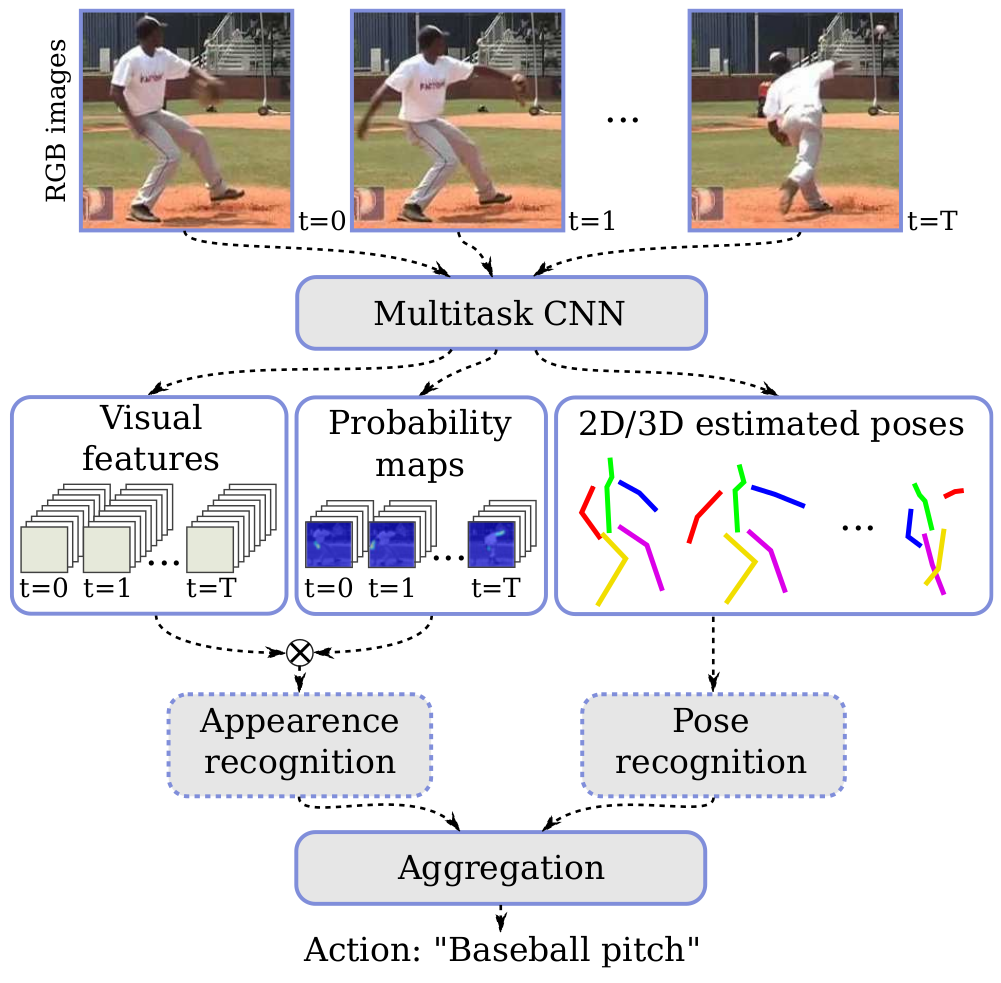
\includegraphics[width=.99\textwidth]{endtoend-concept.png}
            %\caption{Complete network pipeline.}
		\end{figure}
	\end{column}
	\end{columns}
\end{myframe}

\section{Method}
\begin{myframe}[Method]
    \begin{itemize}
        \item Reimplementation in PyTorch \fcite{paszke_automatic_2017}
        \begin{itemize}
            \item Evaluate against HMDB \fcite{kuehne_hmdb:_2011} and Kinetics datasets \fcite{kay_kinetics_2017}
        \end{itemize}
        \item Experimentation
        \begin{itemize}
            \item Better incorporation of temporal dimension \fcite{pavllo_3d_2019}
            \item Compare with state-of-the-art methods not using pose \fcite{zhou_mict:_2018}
        \end{itemize}
    \end{itemize}
\end{myframe}

\section{Datasets}
% also: metrics?
% \begin{myframe}[2D / 3D pose datasets]
%   \begin{itemize}
%       \item \textbf{2D}
%       \begin{itemize}
%           \item MPII \fcite{andriluka_2d_2014}
%           \item LSP \fcite{johnson_clustered_2010}\fcite{johnson_learning_2011}
%       \end{itemize}
%       \item \textbf{3D}
%       \begin{itemize}
%           \item Human 3.6M \fcite{ionescu_human3.6m:_2014}
%       \end{itemize}
%   \end{itemize}
% \end{myframe}

\begin{myframe}[2D pose datasets]
  \begin{columns}[T]
      \begin{column}{.48\textwidth}
          \begin{itemize}
              \item \textbf{MPII Human Pose\footnotemark}
              \begin{itemize}
                  \item 40,000 annotated images
                  \item single and multi person
                  \item over 401 different activities
              \end{itemize}
              \vspace{50px}
              \item \textbf{Leeds Sport Pose \footnotemark \footnotemark}
              \begin{itemize}
                  \item 2,000 pose images, 14 joints
                  \item sport context
                  \item \textbf{LSP-Extended}: Additional 10,000 images
              \end{itemize}
          \end{itemize}
      \end{column}
      \footnotetext[1]{\cite{andriluka_2d_2014}}
      \footnotetext[2]{\cite{johnson_clustered_2010}}
      \footnotetext[3]{\cite{johnson_learning_2011}}
      \begin{column}{.48\textwidth}
          \begin{figure}
              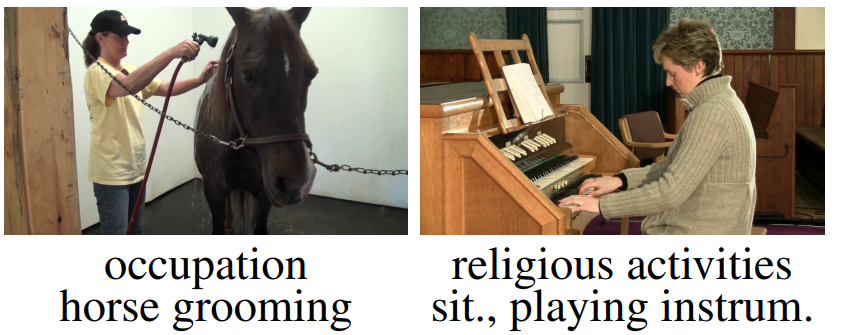
\includegraphics[width=0.99\textwidth]{mpii.png}
          \end{figure}
          \begin{figure}
              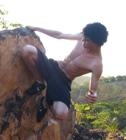
\includegraphics[width=0.48\textwidth]{lsp-original.jpg}
              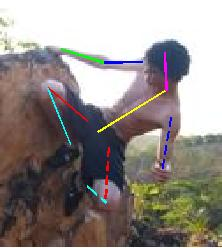
\includegraphics[width=0.48\textwidth]{lsp-annotated.jpg}
          \end{figure}
      \end{column}
  \end{columns}
\end{myframe}

\begin{myframe}[3D pose datasets]
  \begin{columns}[T]
      \begin{column}{.48\textwidth}
          \vspace{50px}
          \begin{itemize}
              \item \textbf{Human3.6m\footnotemark}
              \begin{itemize}
                  \item 3,600,000 annotated images
                  \item annotated using motion capturing system
                  \item 11 male and female actors recreate daily situations
                  \item 17 different scenarios
              \end{itemize}
          \end{itemize}
      \end{column}
      \footnotetext[1]{\cite{ionescu_human3.6m:_2014}}
      \begin{column}{.48\textwidth}
          \begin{figure}
              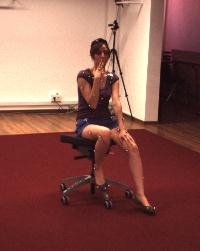
\includegraphics[width=0.48\textwidth]{human-01.jpg}
              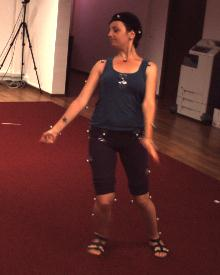
\includegraphics[width=0.48\textwidth]{human-02.jpg}
              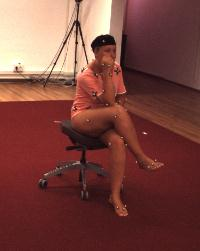
\includegraphics[width=0.48\textwidth]{human-03.jpg}
              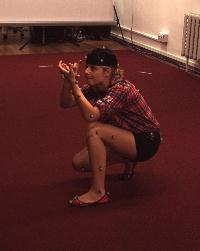
\includegraphics[width=0.48\textwidth]{human-04.jpg}
          \end{figure}
      \end{column}
  \end{columns}
\end{myframe}

% \begin{myframe}[2D HAR datasets]
%   \begin{itemize}
%       \item Penn Action \fcite{zhang_actemes_2013}
%       \item HMDB51 \fcite{kuehne_hmdb:_2011}
%       \item Kinetics \fcite{kay_kinetics_2017}
%   \end{itemize}
% \end{myframe}

\begin{myframe}[2D action recognition datasets]
  \begin{columns}[T]
      \begin{column}{.48\textwidth}
          \vspace{20px}
          \begin{itemize}
              \item \textbf{Penn Action\footnotemark}
              \begin{itemize}
                  \item 2,400 video clips of 15 actions
                  \item very limited number of actions (mainly sport)
              \end{itemize}
              \vspace{40px}
              \item \textbf{Kinetics \footnotemark}
              \begin{itemize}
                  \item 500,000 action-annotated video clips
                  \item 600 classes with at least 600 clips each
                  \item clips from Youtube
                  \item Pitched as the \textit{ImageNet for video}
              \end{itemize}
          \end{itemize}
      \end{column}
      \footnotetext[1]{\cite{zhang_actemes_2013}}
      \footnotetext[2]{\cite{kay_kinetics_2017}}
      \begin{column}{.48\textwidth}
          \begin{figure}
              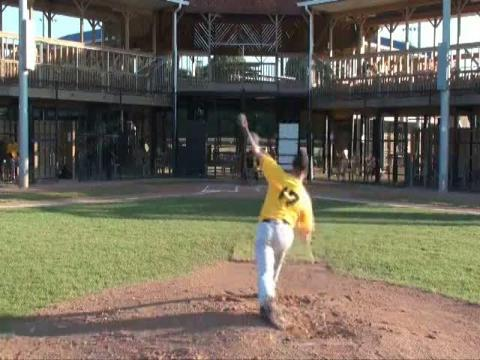
\includegraphics[height=40px]{pa-01.jpg}
              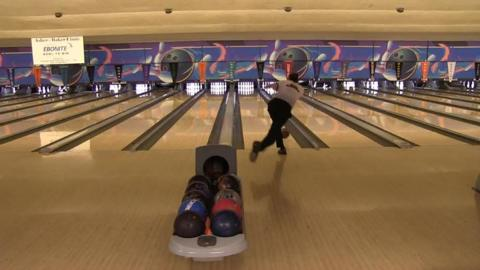
\includegraphics[height=40px]{pa-02.jpg}
              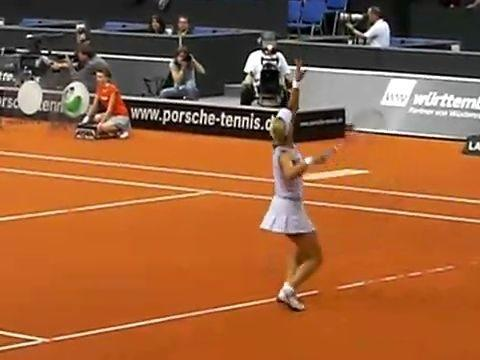
\includegraphics[height=40px]{pa-03.jpg}
              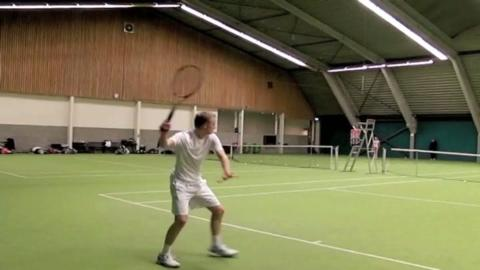
\includegraphics[height=40px]{pa-04.jpg}
          \end{figure}
          \begin{figure}
              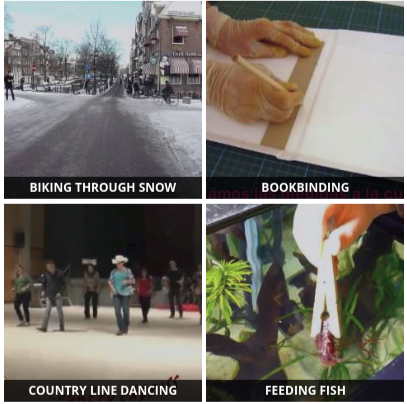
\includegraphics[width=0.69\textwidth]{kinetics-example.png}
          \end{figure}
      \end{column}
  \end{columns}
\end{myframe}

\begin{myframe}[2D action recognition datasets]
  \begin{columns}[T]
      \begin{column}{.48\textwidth}
          \vspace{50px}
          \begin{itemize}
              \item \textbf{HMDB51\footnotemark}
              \begin{itemize}
                  \item 6,800 video clips of 51 actions
                  \item video clips from youtube
                  \item at least 101 clips per action category
              \end{itemize}
          \end{itemize}
      \end{column}
      \footnotetext[1]{\cite{kuehne_hmdb:_2011}}
      \begin{column}{.48\textwidth}
          \begin{figure}
              \includegraphics[height=190px]{hmdb-example.png}
          \end{figure}
      \end{column}
  \end{columns}
\end{myframe}

\begin{myframe}[3D HAR datasets]
  \begin{columns}[T]
      \begin{column}{.48\textwidth}
          \vspace{35px}
          \begin{itemize}
              \item \textbf{NTU RGB+D \footnotemark}
              \begin{itemize}
                  \item 56,000 videos of 60 different actions
                  \item recorded by multiple cameras
                  \item additional depth information
                  \item lab setting
              \end{itemize}
          \end{itemize}
      \end{column}
      \footnotetext[1]{\cite{shahroudy_ntu_2016}}
      \begin{column}{.48\textwidth}
          \begin{figure}
              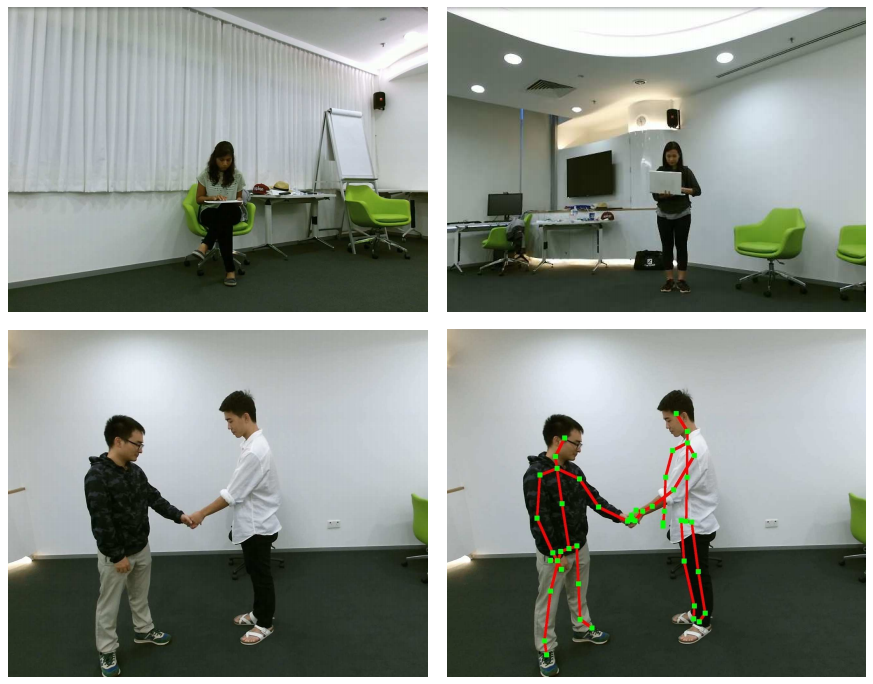
\includegraphics[width=0.99\textwidth]{ntu-example.png}
          \end{figure}
      \end{column}
  \end{columns}
\end{myframe}
\section{Conclusion}
\begin{myframe}[Conclusion]
    \begin{itemize}
        \item Conclusion goes here
    \end{itemize}
\end{myframe}

\begin{myframe}[Thank you]
    \centering \Large
    \emph{Thank you for your time!}
\end{myframe}

\end{document}

